\documentclass{book} 
\usepackage{amsmath,amsthm,amsfonts,float} 
\usepackage{graphicx} 
\usepackage{tikz}
\usetikzlibrary{shapes.geometric}
\numberwithin{equation}{section}

\newtheorem{alevel}{A-LEVEL TASK}
\newtheorem{blevel}{B-LEVEL TASK}
\newtheorem{clevel}{C-LEVEL TASK}
\newtheorem{dlevel}{D-LEVEL TASK}
\newtheorem{elevel}{E-LEVEL TASK}
\theoremstyle{definition}
\newtheorem{bigidea}{BIG IDEA}
\newcommand{\longdiv}{\smash{mkern-0.43mu\vstretch{1.31}{\hstretch{.7}{)}}\mkern-5.2mu\vstretch{1.31}{\hstretch{.7}{)}}}}

%%%%%%%%%%%%%%%%%%%%%%%%%%%%%%%%%%%%%%%%%%%%%%%%%%%%%%%%%


\begin{document}
\title{Learning Electrical Circuit Analysis - Solutions}
\author{Mark Stewart}
\maketitle

%%%%%%%%%%%%%%%%%%%%%%%%%%%%%%%%%%%%%%%%%%%%%%%%%%%%%%%%%%%%%%%%%%%%%%%%
\chapter{Networks - 20 Questions}

\begin{alevel}D has most (4).\end{alevel}

\begin{alevel}See figure.\end{alevel}

\begin{figure}[H]
\begin{center}
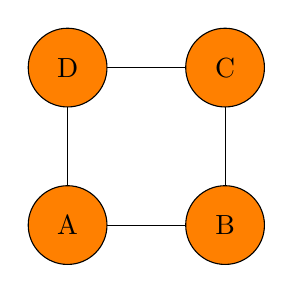
\begin{tikzpicture}
\draw (0,.5)--(0,1.5);
\draw (.5,2)--(1.5,2);
\draw (2,2)--(2,0);
\draw (0,0)--(2,0);
\node[draw,circle,minimum size =1cm, fill=orange] (A) at (0,0){A};
\node[draw,circle,minimum size =1cm, fill=orange] (B) at (2,0){B};
\node[draw,circle,minimum size =1cm, fill=orange] (C) at (2,2){C};
\node[draw,circle,minimum size =1cm, fill=orange] (D) at (0,2){D};
\end{tikzpicture}
\caption{A Friends Network}
\label{F:1FN}
\end{center}
\end{figure}

\begin{alevel}D is friends with 2 people, not 4.\end{alevel}

\begin{alevel}Towns\end{alevel}

\begin{alevel}6 roads, some are two lane\end{alevel}

\begin{alevel}Roads\end{alevel}

\begin{alevel}10 lanes\end{alevel}

\begin{alevel}Can not get to E from B\end{alevel}

\begin{clevel}Yes. EDBAC. Yes, if you start anywhere but E, you can't get to E.\end{clevel}

\begin{dlevel} Can only have two nodes with odd number of roads (Konigsberg Bridge Problem).\end{dlevel}

\begin{alevel}28 miles\end{alevel}

\begin{alevel}E-town\end{alevel}

\begin{alevel}200 $\frac{cars}{min}$\end{alevel}

\begin{clevel}150 entering from A, but 50 leaving to D, so net $+100\frac{cars}{min}$\end{clevel}

\begin{dlevel} Algorthim:\par
\begin{itemize}
\item Label all roads with undetermined flows with a variable.
\item Write an equation for each node that the sum of flows into it sum to zero.
\item Solve this simultaneous set of equations.
\end{itemize}
\end{dlevel}

\begin{alevel} A to D\end{alevel}
\begin{blevel} +6 mi\end{blevel}
\begin{clevel} 0, yes\end{clevel}

\begin{blevel}1 gall = 3.78 kg, so 37.8 kg/s.\end{blevel}

\begin{blevel}It would increase at 2 gal/s. The water would need to be stored inside J1 (maybe compressed?).\end{blevel}

\begin{clevel}$\frac{Vol}{sec}=\frac{Area*length}{s}=\frac{0.000628m^3}{s} \rightarrow 9.97 gal/s$\end{clevel}

\begin{alevel}Neurons or little computers.\end{alevel}
\begin{blevel}$5*1+10*2=25 > 5$ therefore out=1\end{blevel}
\begin{clevel}$5*C3+2*C2-5*C1=5-2-5=-1$\end{clevel}
\begin{clevel}No way. Outflow will always be 1 or -1.\end{clevel}

 %%%%%%%%%%%%%%%%%%%%%%%%%%%%%%%%%%%%%%%%%%%%%%%%%%%%%%%%%%%%%%%%%%%%%%%%%%%%%%%%%
\setcounter{alevel}{0} \setcounter{blevel}{0} \setcounter{clevel}{0} \setcounter{dlevel}{0}
\chapter{Electrical Networks 84 Questions}
\begin{blevel}Table.\par
\begin{table}[H]
\begin{center}
\begin{tabular}{|c|c|} \hline
particle	&	charge (units of $e^-$) \\ \hline
electron	&	-1\\ \hline
proton		&	+1\\ \hline
top quark	&	$\frac{2}{3}$\\ \hline
muon		&	-1\\ \hline
neutron		&	0\\ \hline
photon		&	0\\ \hline
Sodium Ion	&	+1\\ \hline
\end{tabular}
\caption{Summary of amount of charge that some particles have}
\label{T:2EP}
\end{center}
\end{table}
\end{blevel}

\begin{alevel}Coulombs\end{alevel}
\begin{blevel}$\frac{1}{1.6E-19}=6.25E18$ electrons\end{blevel}
\begin{alevel}5 C each second. 300 C each minute.\end{alevel}
\begin{blevel}3.125E19 each second, 1.875E21 each minute.\end{blevel}

\begin{blevel}Table.\par
\begin{table}[H]
\begin{center}
\begin{tabular}{|c|c|c|c|} \hline
item	&	abbreviation & units & units abbreviation \\ \hline
Force	&	F	& Newton	& N\\ \hline
mass	&	m	& kilogram	&	kg	\\ \hline
charge	& q	& Coulomb& C	\\ \hline
current		&I&Amp&A	\\ \hline
temperature		&T&$^\circ$Celsius&$^\circ$C	\\ \hline
Energy	&E&Joule&J	\\ \hline
Power	&P&Watt&W	\\ \hline
\end{tabular}
\caption{Symbols and units}
\label{F:2SU}
\end{center}
\end{table}
\end{blevel}

\begin{alevel}2.5$\frac{m}{s}$\end{alevel}
\begin{blevel}Can't tell.\end{blevel}
\begin{dlevel}Can't tell because we don't know the position at any time. Velocity can't determine position, only change in position.\end{dlevel}
\begin{blevel}$\bar{a}=\frac{2.5-1}{4-0}=0.375\frac{m}{s^2}$\end{blevel}
\begin{blevel}0\end{blevel}
\begin{blevel}Use tangent: $a=\frac{2.5-1}{4-2}=0.75\frac{m}{s^2}$\end{blevel}

\begin{clevel} Graph.\par
\begin{figure}[H]
\begin{center}
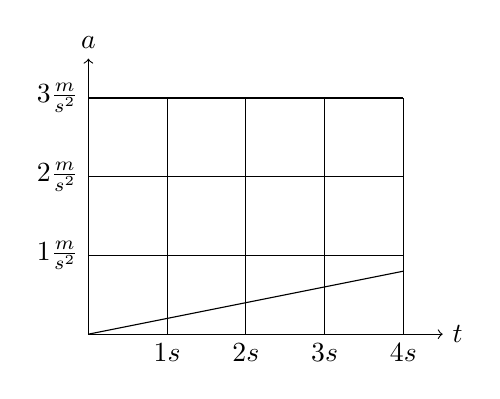
\begin{tikzpicture}
\draw[->] (0,0)--(4.5,0) node[right] {$t$};
\draw[->] (0,0)--(0,3.5) node[above] {$a$};
\draw (0,1)node[left] {$1 \frac{m}{s^2}$} --(4,1);
\draw (0,2)node[left] {$2 \frac{m}{s^2}$}--(4,2) ;
\draw (0,3)node[left] {$3 \frac{m}{s^2}$}--(4,3) ;
\draw (1,0)node[below] {$1 s$}--(1,3) ;
\draw (2,0)node[below] {$2 s$}--(2,3) ;
\draw (3,0)node[below] {$3 s$}--(3,3) ;
\draw (4,0)node[below] {$4 s$}--(4,3) ;
\draw [smooth, samples=100,domain=0:4] plot(\x,{.2*(\x)});
\end{tikzpicture}
\caption{The car's acceleration as a function of time.}
\label{F:2CAR}
\end{center}
\end{figure}
\end{clevel}

\begin{alevel}2.5C\end{alevel}
\begin{blevel}0.375A\end{blevel}
\begin{blevel}0.75A\end{blevel}
\begin{clevel}same as Figure~\ref{F:2CAR}, but with units of Amps\end{clevel}
\begin{alevel}$\frac{1}{s}$\end{alevel}

\begin{clevel} Given: $i=3q+1$ \par
\begin{align*}
\frac{dq}{dt}&=3q+1\\
\frac{dq}{3q+1}&=dt\\
\int\limits_5^Q{\frac{dq}{3q+1}}&=\int\limits_0^t{dt}\\
ln(3Q+1)-ln(16)&=3t\\
Q=\frac{16e^{3t}-1}{3}
\end{align*}
\end{clevel}
\begin{clevel}$i=6e^{2t}$\end{clevel}

\begin{clevel} Table\par
\begin{table}[H]
\begin{center}
\begin{tabular}{|c| c| c|} \hline
item & relevant formula	& rough value \\ \hline
stand up	& W = F*d	& $(100kg)*(9.8 \frac{m}{s^2})*.5 m \approx 500J$\\ \hline
heat up cup of coffee &$Q=mc\Delta T$	& $0.5*4186*80=160000J$\\ \hline
start running sideways	&$KE=\frac{1}{2}mv^2$	&50J\\ \hline
drag a log 20 feet	&$W=F*d$	&500*6 = 3000J\\ \hline
create a 1kg of mass	&$E=mc^2$	&3E18 J\\ \hline
create one photon ($\lambda$=650 nm)	&$E=\frac{hc}{\lambda}$	&3.06E-19J	\\ \hline
case A*			&$W=\int{F\bullet dx}$	&$W=\int\limits_4^2{\frac{-kq_eq_e}{x^2}\bullet dx}$=5.76e-29J\\ \hline
case B*			&$W=\int{F\bullet dx}$	&$W=\int\limits_2^4{\frac{G(1)(1)}{x^2}\bullet dx}$=1.67E-11J\\ \hline
\end{tabular}
\caption{Approximate amount of energy needed to do several tasks.}
\end{center}
\end{table}
\end{clevel}

\begin{blevel}Energy can be transformed from one form to another, but not created or destroyed in a closed system.\end{blevel}
\begin{alevel}Trails\end{alevel}
\begin{blevel}Yes, their elevations above some reference point.\end{blevel}
\begin{alevel}0\end{alevel}
\begin{blevel}Any loop starting and ending at the same spot with have a net height change of zero.\end{blevel}
\begin{blevel}$\Delta PE_{Comet}=24500J$,$\Delta PE_{Ajax}=39200J$, but per mass both are 490 $\frac{J}{kg}$\end{blevel}

\begin{blevel} Table\par
\begin{table}[H]
\begin{center}
\begin{tabular}{|c|c|}\hline
pts&Grav. Potential ($V_G$)\\ \hline
$V_{AB}$& +294$\frac{J}{kg}$\\ \hline
$V_{AC}$& -490$\frac{J}{kg}$\\ \hline
$V_{CE}$& +490$\frac{J}{kg}$\\ \hline
$V_{CD}$& 0\\ \hline
$V_{EC}$& -490$\frac{J}{kg}$\\ \hline
\end{tabular}
\caption{Values for gravitational potential energy per mass (gravitational potential)}
\label{T:2GP}
\end{center}
\end{table}
\end{blevel}

\begin{clevel}NO!\end{clevel}
\begin{blevel}$\frac{J}{kg}$\end{blevel}
\begin{blevel}22.5J\end{blevel}
\begin{alevel}NO!\end{alevel}
\begin{blevel}$V=\frac{PE_{electrical}}{q}$\end{blevel}


\begin{alevel}No, just transforms it from one form to another.\end{alevel}
\begin{alevel}$\frac{Energy}{sec}=\frac{J}{s}$\end{alevel}
\begin{blevel}7500J\end{blevel}
\begin{clevel}$\approx$ 67000 W\end{clevel}
\begin{alevel}$\approx$ 746J\end{alevel}

\begin{blevel}39.2$\frac{J}{kg}$ difference\end{blevel}
\begin{blevel}1510 Watts\end{blevel}
\begin{blevel}$\frac{C}{s}*\frac{J}{C}=\frac{J}{s}$\end{blevel}
\begin{clevel}$\frac{60.96m*9.8*.37.8kg}{60s}=376W$\end{clevel}
\begin{clevel}$\frac{0.436m*9.8*1000}{s}=4270W$\end{clevel}
\begin{blevel}1800 Joules each minute\end{blevel}
\begin{alevel}photon\end{alevel}
\begin{blevel}$\frac{300}{0.19}/1000=1.58m^2$\end{blevel}
\begin{blevel}3240000J\end{blevel}
\begin{blevel}6.25A\end{blevel}
\begin{blevel}about 373 panels\end{blevel}

\begin{blevel}Table.\par
\begin{table}[H]
\begin{center}
\begin{tabular}{|c|c|c|}\hline
which points	& Voltage (Arrangement 1)&Voltage (Arrangement 2) \\ \hline
BC & 48V& 48V\\ \hline
CB & -48& -48V\\ \hline
AB & 0& 0\\ \hline
BD & 96V& 48V\\ \hline
DE & -96V& -48V\\ \hline
DA & -96V& -48V\\ \hline
AD & +96V& +48V\\ \hline
FD & n/a &+48V \\ \hline	
\end{tabular}
\end{center}
\end{table}
\end{blevel}

\begin{blevel}6.25A\end{blevel}

\begin{blevel} Table.\par
\begin{table}[H]
\begin{center}
\begin{tabular}{|c|c|c|}\hline
which current	& Current (Arrangement 1)&Current (Arrangement 2) \\ \hline
I1 & -6.25A& -12.5A\\ \hline
I2 & 6.25A& -6.25A\\ \hline
I3 & -6.25A& -12.5A\\ \hline
\end{tabular}
\label{T:2SSC}
\end{center}
\end{table}
\end{blevel}

\begin{blevel}First case: 96V, 6.25A, 600W. Second case: 48V, 12.5A, 600W.\end{blevel}
\begin{clevel}Two strings of 4 in parallel.\end{clevel}

\begin{alevel}200J\end{alevel}
\begin{blevel}Because Watt is already a rate. Does this mean they install 500W each day?\end{blevel}
\begin{blevel}3600000J\end{blevel}
\begin{blevel}1.5kWhr\end{blevel}
\begin{blevel}about 30\end{blevel}
\begin{blevel}234MJ, \$13 to charge\end{blevel}
\begin{blevel}1200W, 54.2 hours\end{blevel}
\begin{blevel}about 20 minutes\end{blevel}

\begin{blevel} Table.\par
\begin{table}[H]
\begin{center}
\begin{tabular}{ |c | c | c | c |} \hline
network	&	what are nodes	& what are edges	& what flows \\ \hline
friends	&	people	& indications of friendship	& n/a \\ \hline
traffic &	towns	& roads				&cars	\\ \hline
water	&	junctions	& pipes				&water	\\ \hline
electrical	& places of equal electrical energy	& wires, resistors	&electrical charge, probably electrons	\\ \hline
\end{tabular}
\caption{Network Summary Table}
\end{center}
\end{table}
\end{blevel}

\begin{alevel}$\frac{J}{C}$ or $\frac{Nm}{C}$\end{alevel}
\begin{alevel}$\frac{J}{kg}$ or $\frac{Nm}{kg}$\end{alevel}
\begin{blevel}$\vec{F}=30N\hat{j}$ then $\vec{a}=10\frac{m}{s^2}\hat{j}$\end{blevel}
\begin{blevel}$\vec{F}=-10N\hat{i}+30N\hat{j}$ then $|\vec{a}|=10.54\frac{m}{s^2}$\end{blevel}
\begin{blevel}higher at (0,0) because field would pull mass to the right\end{blevel}
\begin{clevel}+15J\end{clevel}
\begin{clevel}+1.5$\frac{J}{kg}$\end{clevel}
\begin{clevel}+10V, higher at (0,0)$\frac{J}{kg}$\end{clevel}

%%%%%%%%%%%%%%%%%%%%%%%%%%%%%%%%%%%%%%%%%%%%%%%%%%%%%%%%%%%%%%%%%%%%%%%%%%%%%
\setcounter{alevel}{0} \setcounter{blevel}{0} \setcounter{clevel}{0} \setcounter{dlevel}{0}
\chapter{Basic Components}

\begin{blevel}Case 1 has person touching the case and the +wire touching case, but the breaker is already tripped.\end{blevel}
\begin{alevel}Light emitting diode\end{alevel}
\begin{blevel}A two-terminal device usually associated with assymetrical behavior, like a one-way valve.\end{blevel}
\begin{alevel}500 or 600 Celsius\end{alevel}
\begin{alevel}behaving like a voltage source\end{alevel}
\begin{blevel}no change, still 10A\end{blevel}
\begin{alevel}Voltage\end{alevel}
\begin{alevel}Ohms\end{alevel}
\begin{clevel}$\Omega=\frac{Js}{C^2}$\end{clevel}
\begin{clevel}$\Omega=\frac{kg*m^2}{s*C^2}$\end{clevel}
\begin{blevel}hack,hack,always good (definition), hack\end{blevel}

\begin{blevel}Table\par
\begin{table}[H]
\begin{center}
\begin{tabular}{|c|c|c|}\hline
item&answer&hints\\ \hline
$I_1$	&-3A	&	\\ \hline
$V_{AB}$	&0	&	\\ \hline
$V_{BC}$	&+15V	& use Ohm's law	\\ \hline
$V_{AD}$	&+15V	&	\\ \hline
$I_{from B to C}$	&3A	&	\\ \hline
Power absorbed by R	&45W	&	\\ \hline
Power produced by current source	&45W	&	\\ \hline
\end{tabular}
\label{T:21}
\caption{Summary of select parameters for simple circuit.}
\end{center}
\end{table}
\end{blevel}

\begin{blevel}12-gauge: $A=3.31mm^2$, $R=\frac{1.68E-8*20}{3.31E-6}= 0.101 \Omega$\end{blevel}
\begin{blevel}$R=\frac{2.65E-8*.005}{1E-13}= 1325 \Omega$, V=132.5V, P=13.25W\end{blevel}
\begin{dlevel}
\begin{align*}
mass=\rho*Volume=1.35E-12kg\\
\Delta Q=13.25*60=795J\\
\Delta T=\frac{Q}{mc}=\frac{795J}{1.35E-12kg*920\frac{J}{kgC}}=6.4E11 ^\circ C\\
T_{melt}=\frac{Q_{melt}}{P_{in}}=\frac{7.5E-8J+5.1E-10J}{13.25W}\approx 6ns
\end{align*}
\end{dlevel}
\begin{blevel}A=3.31E-6 $m^2$, k=398 W/mK, so Q= 60s*0.044J/s=2.64 J/min\end{blevel}
\begin{blevel}A=3.31E-6 $m^2$, $\rho$=1.72E-8 $\Omega m$, so Q= 60s*3460 A so Q=207,000 C/min\end{blevel}


%%%%%%%%%%%%%%%%%%%%%%%%%%%%%%%%%%%%%%%%%%%%%%%%%%%%%%%%%%%%%%%%%%%%%%%%%%%%%%%%%%%%%%%%
\setcounter{alevel}{0} \setcounter{blevel}{0} \setcounter{clevel}{0} \setcounter{dlevel}{0}
\chapter{Basic Tools.}

\begin{blevel}$20+5*120-7*60=200 Amps$ therefore out=1\end{blevel}
\begin{dlevel}No, mass and energy can be converted back and forth. It should work for the cafeteria if food in stomachs and trash were considered\end{dlevel}
\begin{blevel} options
\begin{itemize}
\item No, gasoline to exhaust.
\item Yes.
\item Yes, but only over time.
\item Yes.
\end{itemize}\end{blevel}

\begin{alevel}5V\end{alevel}
\begin{alevel}15 Joules of heat\end{alevel}

\begin{blevel}$I_1=1A,I_5=0.5A,V_{AD}=2.5V$\end{blevel}
\begin{clevel}12.5V\end{clevel}
\begin{clevel}Table\par
\begin{table}[H]
\begin{center}
\begin{tabular}{|c|c|c|c|} \hline
component &	current through it	& voltage across it	& power consumed \\ \hline
2A source	&+2A			&-13V (V, I in opp. dirs.)	&-26Watts\\ \hline
3A source	&3A			&12.5V	&-37.5W	\\ \hline
10 Ohm (E-F)	&+2A			&+20V	&+40W	\\ \hline
5 Ohm (B-C)	&+1A			&+5V	&+5W	\\ \hline
10 Ohm (G-D)	&0.7A			&+7V	&+4.9W	\\ \hline
1 Ohm (A-D)	&2.5A			&-2.5V	&+6.25W	\\ \hline
5 Ohm (A-D)	&0.5A			&-2.5V	&+1.25W	\\ \hline
5V source	&2.3A			&5V	&+11.5W	\\ \hline
Gator Top	&2A			&2V	&-4W	\\ \hline
Gator Side	&.7A			&2V	&-1.4W	\\ \hline
\end{tabular}
\caption{Table to check conservation of energy.}
\label{F:3CKT3}
\end{center}
\end{table}
\end{clevel}

\begin{clevel}$P_{Total}=68.9W-68.9W=0$\end{clevel}

\begin{clevel}Table\par
\begin{table}[H]
\begin{center}
\begin{tabular}{|c|c|c|c|} \hline
component &	current through it	& voltage across it	& power consumed \\ \hline
2A source	&+2A			&-8V (V, I in opp. dirs.)	&-16Watts\\ \hline
3A source	&3A			&30V	&-90W	\\ \hline
10 Ohm (E-F)	&+2A			&+20V	&+40W	\\ \hline
5 Ohm (B-C)	&+1A			&+10V	&+10W	\\ \hline
10 Ohm (G-D)	&0.7A			&+7V	&+4.9W	\\ \hline
1 Ohm (A-D)	&1.5A			&-15V	&+22.5W	\\ \hline
5 Ohm (A-D)	&1.5A			&-15V	&+22.5W	\\ \hline
5V source	&2.3A			&5V	&+11.5W	\\ \hline
Gator Top	&2A			&2V	&-4W	\\ \hline
Gator Side	&.7A			&2V	&-1.4W	\\ \hline
\end{tabular}
\caption{Table to check conservation of energy. 111.4W=111.4W}
\label{F:3CKT3}
\end{center}
\end{table}
\end{clevel}

\begin{alevel} 8 $\Omega$ \end{alevel}

\begin{clevel}$V_T=IR_1+IR_2+IR_3 = I(R_1+R_2+R_3) \rightarrow V_T=IR_T$\\
therefore $R_T=R_1+R_2+R_3$
\end{clevel}

\begin{alevel} $\frac{15}{8} \Omega$ \end{alevel}

\begin{clevel}\begin{align*}
R_T&=R_1+R_2\\
\rho\frac{L}{A}&=\rho\frac{L_1}{A}+\rho\frac{L_2}{A}\\
L&=L_1+L_2
\end{align*}
\end{clevel}

\begin{clevel}In parallel: $I_T=\frac{V}{R_1}+\frac{V}{R_2} = V(\frac{1}{R_1}+\frac{1}{R_2}) \rightarrow I_T=\frac{V}{R_T}$\\
therefore $\frac{1}{R_T}=\frac{1}{R_1}+\frac{1}{R_2}$
\end{clevel}


\begin{clevel} \begin{align*}
\frac{1}{R_T}&=\frac{1}{R_1}+\frac{1}{R_2}\\
\frac{A}{\rho L}&=\frac{A_1}{\rho L}+\frac{A_2}{\rho L}\\
A&=A_1+A_2
\end{align*}
\end{clevel}

\begin{clevel} \begin{align*}
\frac{1}{R_T}&=\frac{1}{R_1}+\frac{1}{R_2}\\
\frac{1}{R_T}&=\frac{R_2}{R_1R_2}+\frac{R_1}{R_1R_2}\\
R_T&=\frac{R_1R_2}{R_1+R_2}
\end{align*}
\end{clevel}

\begin{blevel} $\frac{\Omega^3}{\Omega} \neq \Omega$
\end{blevel}

\begin{blevel} resistance will go Down\end{blevel}

\begin{dlevel} $R_T=\frac{S_N}{S_{N-1}}$\end{dlevel}

\begin{clevel} Table\par 
\begin{table}[H]
\begin{center}
\begin{tabular}{|c|c|} \hline
components & series, parallel or neither \\ \hline
X and W & parallel	\\ \hline
Z and W &neither	\\ \hline
Y and M &neither	\\ \hline
N and M &series	\\ \hline
Z and Y &parallel	\\ \hline
X and M &neither	\\ \hline
\end{tabular}
\caption{Series or parallel?}
\label{T:3SP}
\end{center}
\end{table}
\end{clevel}

\begin{clevel}30 $\Omega$\end{clevel}
\begin{blevel} Drawing of circuit: $(X \parallel (W+Z)+A)\parallel Y+M$\end{blevel}


\begin{blevel}$5+5\parallel 5$\end{blevel}
\begin{alevel}harder\end{alevel}
\begin{clevel} 
\begin{align*}
R_T=R+R\parallel R_T=R+\frac{RR_T}{R+R_T}\\
R_T^2+R_TR=R_TR+R^2+RR_T\\
R_T^2-RR_T-R^2=0\\
R_T=R(\frac{1+\sqrt{5}}{2})
\end{align*}
\end{clevel}
\begin{blevel}2.2 Siemens\end{blevel}
\begin{blevel}12.875 Distrusters\end{blevel}
\begin{clevel}3.6 Distrusters\end{clevel}
\begin{blevel}$\frac{1}{Lyes}$\end{blevel}

\begin{clevel}0.0776 Trust, yes, consistent because this is inverse of distrust\end{clevel}

\begin{clevel}Current sources would add in parallel, but different ideal current sources would be a catastrophe in series.\end{clevel}
\begin{blevel}It is made of copper because of the resistivity value.\end{blevel}
\begin{blevel}$R=\frac{15.46\Omega}{3}=5.15 \Omega \rightarrow R_T=5.64\Omega$\\
$V_{SAW}=115-2*.246*\frac{115}{5.64}=104.96V$\end{blevel}
\begin{clevel}$\frac{R}{N}$\end{clevel}
\begin{clevel}$R_{SAW}=\frac{115^2}{P}, R_{cord}=L*.00807 \frac{\Omega}{m}$\\
$R=\frac{\frac{115^2}{P}}{N}\Omega \rightarrow R_T=\frac{115^2}{PN}+2*L*.00807 \Omega $\\
$V_{SAW}=115-2*L*.00807*\frac{115}{\frac{115^2}{PN}+2*L*.00807}$
Should be simplified or use voltage division (next section) to get simpler result.
\end{clevel}

%%springs
\begin{alevel} Stretches $\frac{10}{k_3}$\end{alevel}
\begin{clevel} 
\begin{align*}
\Delta x_T&=\Delta x_1+\Delta x_2\\
\frac{F}{k_T}&=\frac{F}{k_1}+\frac{F}{k_2}\\
\frac{1}{k_T}&=\frac{1}{k_1}+\frac{1}{k_2}
\end{align*}
\end{clevel}
\begin{blevel}$k_{eq}=\frac{70}{17}$ N/m, $\Delta x=\frac{51}{70}$ m\end{blevel}

%%tasks
\begin{blevel}$t=3\frac{5}{6}$ hrs\end{blevel}
\begin{blevel}$t=2.49$ hrs\end{blevel}


\begin{alevel}$V_{R1}=6V$,$V_{R2}=12V$\end{alevel}
\begin{blevel}$V_{AB}+V_{BC}=18V$\\
$V_{AB}+V_{BA}=0$\\
$V_{AB}+V_{CB}=-6V$
\end{blevel}
\begin{dlevel}$V_i=\frac{R_i}{R_i+R_{remaining}}=..$\end{dlevel}
\begin{blevel}1.47V\end{blevel}
\begin{clevel}3.68V\end{clevel}
\begin{clevel}2.21V\end{clevel}

%%%%%%%%%%%%%%%%%%%%%%%%%%%%%%%%%%%%%%%%%%%%%%%%%%%%%%%%%%%%%%%%%%%%%%%%%%%%%%
\setcounter{alevel}{0} \setcounter{blevel}{0} \setcounter{clevel}{0} \setcounter{dlevel}{0}
\chapter{Powerful Tools}

\begin{alevel}N=3 equations, M=2 unknowns\end{alevel}
\begin{blevel}infinite solutions\end{blevel}
\begin{clevel}x=a, y=10-a or 
$\left[ \begin{matrix}x\\y \end{matrix}\right]=
\left[ \begin{matrix}10\\0 \end{matrix}\right]+
a\left[ \begin{matrix}1\\-1 \end{matrix}\right]$
\end{clevel}

\begin{dlevel}form a matrix and check its determinant. If it equals 0, then they are not independent.\end{dlevel}

\begin{blevel} $\left[ \begin{matrix}0\\30 \end{matrix}\right]$ \end{blevel}
\begin{blevel} $\left[ \begin{matrix}a&b\\c&d \end{matrix}\right]$ \end{blevel}
\begin{blevel} $\left[ \begin{matrix}1&0\\0&1 \end{matrix}\right]=I$ \end{blevel}
\begin{blevel} $\left[ \begin{matrix}1&0\\0&1 \end{matrix}\right]=I$, yes, because that is what an inverse does..it undoes multiplying by M \end{blevel}
\begin{blevel} \begin{align*}
&=M^{-1}M^{-1}M^{-1}M^{-1}MMMMM\\
&=M^{-1}M^{-1}M^{-1}(M^{-1}M)MMMM\\
&=M^{-1}M^{-1}M^{-1}(I)MMMM\\
&=M^{-1}M^{-1}M^{-1}MMMM \rightarrow = M
\end{align*}
\end{blevel}
\begin{blevel} $\left[ \begin{matrix}-6&7\\-8&-6 \end{matrix}\right]=I$ \end{blevel}
\begin{clevel}MxN can only be multiplied by RxC is N=R. The result will be a MxC matrix.\end{clevel}
\begin{blevel} $\left[ \begin{matrix}-5&-3.5&-2.5\\-3.5&-4.55&-3.25\\-2.5&-3.25&-3.75 \end{matrix}\right]$ \end{blevel}
\begin{clevel} $\left[ \begin{matrix}3V\\12.9V\\13.5V \end{matrix}\right]$ 
\end{clevel}
\begin{blevel} $I=\frac{C-B}{3}=\frac{9.9}{3}=3.3A$, P=32.7W \end{blevel}

\begin{clevel} Table\par
\begin{table}[H]
\begin{center}
\begin{tabular}{|c|c|c|c|} \hline
component & I&$\Delta V$&power absorbed (- if produced) \\ \hline
3 $\Omega$ &3.3A&9.9V&+32.67W	\\ \hline
2 $\Omega$&-.3A&-.6V&+0.18W	\\ \hline
10 $\Omega$ &0.3A&3V&+0.9W	\\ \hline
5 $\Omega$ &2.7A&13.5V&+36.45W	\\ \hline
3A left source &3A&12.9V&-38.7W	\\ \hline
3A center source &3A&10.5W&-31.5W	\\ \hline
\end{tabular}
\caption{Power check: -70.2W=70.2W}
\label{T:4PCheck}
\end{center}
\end{table}
\end{clevel}

\begin{clevel} $\left[ \begin{matrix}0\\30V\\30V \end{matrix}\right]$ 
\end{clevel}
\begin{clevel} $\left[ \begin{matrix}14.7\\14.07V\\7.67V\\-1.67A \end{matrix}\right]$ 
\end{clevel}
\begin{alevel} Easier to handle current sources. \end{alevel}

\begin{clevel} Equations\par
\begin{align}
\frac{C-B}{3}+\frac{0-B}{10}-I_1=0 \tag{Node B}\\
I_2 + \frac{B-C}{3}+\frac{D-C}{2}=0 \tag{Node C}\\
\frac{C-D}{2}+I_1+\frac{0-D}{5}=0 \tag{Node D}\\
B=D+7 \tag{Bonus Equation due to 7V Voltage Source}\\
C=3 \tag{Bonus Equation due to 3V Voltage Source}
\end{align} 
Answers:$\left[ \begin{matrix}B=6.53V\\C=3V\\D=-.47V\\I_1=-1.83A\\I_2=0.559A \end{matrix}\right]$ 
\end{clevel}

\begin{clevel} 3+(9-1)=11 equations or rows\end{clevel}
\begin{clevel} 3+(25-1)=27 equations or rows\end{clevel}

\begin{alevel} 5 rectangles\end{alevel}
\begin{blevel} 7 polygons\end{blevel}
\begin{clevel} 3 primitive polygons \end{clevel}

\begin{blevel} $\left[ \begin{matrix}-0.22&-0.13&-.15\\-0.13&-0.28&-0.088\\-.15&-0.088&-0.165 \end{matrix}\right]$ \end{blevel}
\begin{clevel} $\left[ \begin{matrix}I_1=0.56A\\I_2=1.74A\\I_3=-.094A \end{matrix}\right]$ \end{clevel}
\begin{clevel} when switched..$\left[ \begin{matrix}I_1=0.76A\\I_2=-.94A\\I_3=0.98A \end{matrix}\right]$ \end{clevel}
\begin{dlevel} The 3V source is on the outer edge of the graph and therefore is in one loop, the 7V source is on an inside edge and is shared by two loops. For a planar network (assumption), it can only appear twice.\end{dlevel}
\begin{dlevel} Equations would no longer be independent.\end{dlevel}

\begin{clevel} 
\begin{align*}
\text{First Loop (A-C-B-A):}&&+3-3(I_1-I_2)-10(I_1-I_3)&=0\\
\text{Second Loop (B-C-D-B):}&&-3(I_2-I_1)-2I_2+V_x&=0\\
\text{Third Loop (A-B-D-A):}&&-10(I_3-I_1)-V_x-5I_3&=0\\
\text{Current Source Bonus Eq:}&&I_3-I_2&=3A
\end{align*}

In matrix form:
\begin{align}
\left[ \begin{matrix}
(-3-10)&3&10&0\\3&(-3-2)&0&1\\10&0&(-10-5)&-1\\0&-1&1&0\\
\end{matrix} \right]
\left[ \begin{matrix}I_1\\I_2\\I_3\\V_x\end{matrix} \right] =
\left[ \begin{matrix}-3\\0\\0\\3\end{matrix} \right]
\end{align}
Solution (Vx could have either sign):$\left[ \begin{matrix}0.82A\\-1.71A\\1.29A\\-11.04V\end{matrix} \right]$
\end{clevel}

\begin{clevel} Loop analysis would be easier with more voltage sources. \end{clevel}
\begin{clevel} 5+1=6 \end{clevel}
\begin{blevel} $B=\frac{\mu_o I}{2\pi r}=3.33E-5 T$ \end{blevel}
\begin{clevel} $P=IV=\frac{V^2}{R_1} \rightarrow lim_{R_1 \rightarrow 0}P=\infty$ \end{clevel}
\begin{blevel} $I=\frac{V}{R_1}$\end{blevel}
\begin{blevel} 7.89V\end{blevel}
\begin{blevel} $V_1=\frac{R_1}{R_{in}+R_1}V$\end{blevel}
\begin{clevel} $R_1=R_{in}$\end{clevel}
\begin{alevel} $I=\frac{5}{1+R}$\end{alevel}
\begin{clevel} $I=\frac{5}{1+R}$\end{clevel}

\begin{alevel} Figure\par 
\begin{figure}[H]
\begin{center}
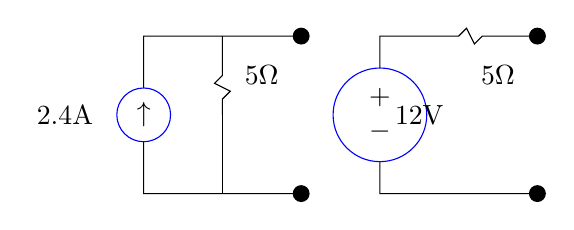
\begin{tikzpicture}
\draw (1,0)--(-1,0)--(-1,1)node[circle, draw=blue, fill=white]{$\uparrow$}--(-1,2)--(0,2)--(0,1.5)--(-.1,1.4)--(.1,1.3)--(0,1.2)--(0,1) (0,2)--(1,2);
\draw  (0,1)--(0,0);
\draw node at (.5,1.5) {$5 \Omega$};
\draw node at (-2,1) {2.4A};
\filldraw (1,2) circle[radius=1 mm];
\filldraw (1,0) circle[radius=1 mm];

\draw (4,0)--(2,0)--(2,1)node[circle, draw=blue, fill=white]{$\begin{matrix}+\\-\end{matrix}$}--(2,2)--(3,2)--(3.1,2.1)--(3.2,1.9)--(3.3,2)--(4,2);
\draw node at (3.5,1.5) {$5 \Omega$};
\draw node at (2.5,1) {12V};
\filldraw (4,2) circle[radius=1 mm];
\filldraw (4,0) circle[radius=1 mm];
\end{tikzpicture}
\caption{Both versions}
\label{F:4NOR}
\end{center}
\end{figure}
\end{alevel}

\begin{blevel} Table\par
\begin{table}[H]
\begin{center}
\begin{tabular}{|c|c|} \hline
Th\'{e}venin version & Norton Version \\ \hline
$W_V=(30V,10\Omega)$&$W_N=(3A,10\Omega)$ \\ \hline
$W_V=(3V,10\Omega)$&$W_N=(0.3A,10\Omega)$ \\ \hline
$W_V=(12V,5\Omega)$&$W_N=(2.4A,5\Omega)$ \\ \hline
\end{tabular}
\end{center}
\end{table}
\end{blevel}

\begin{blevel}$(W+Y)_T=(1V,12\Omega)$\end{blevel}
\begin{clevel}$(W+Y)_T=(28V,12\Omega)$\end{clevel}
\begin{clevel}$I_5=0.79A$ note that 7V is now backwards\end{clevel}
\begin{alevel}\$120 per hour\end{alevel}
\begin{blevel}20.5V\end{blevel}
\begin{clevel}58V\end{clevel}
\begin{alevel}\$180,\$180\end{alevel}
\begin{blevel}5.34V\end{blevel}
\begin{clevel}
\[
V_{out}=\underbrace{\underline{5V}}_{7V}+\underbrace{\underline{-4.28V}}_{3A} = 0.72V
\]
\end{clevel}

\begin{blevel}161.5N\end{blevel}
\begin{clevel}$\frac{16}{5}*24.5+\frac{25}{10}*68.5=249.7N$\end{clevel}

\begin{clevel} Let $R_x=5\parallel(2\parallel 10 +3) = 2.414\Omega$\\
$V_2=(\frac{2\parallel 10}{2\parallel 10 + 3})(\frac{R_x}{R_x+7})5=0.458V$\\
So $I=\frac{0.458V}{2}=0.229A$
\end{clevel}
\begin{clevel}
$V_2=(\frac{2\parallel 10}{2\parallel 10 + 3+7\parallel 5})5=1.538V$\\
So $I=\frac{1.538V}{2}=0.769A$
\end{clevel}

%%%%%%%%%%%%%%%%%%%%%%%%%%%%%%%%%%%%%%%%%%%%%%%%%%%%%%%%%%%%%%%%%%%%%%%%%%%%%%
\setcounter{alevel}{0} \setcounter{blevel}{0} \setcounter{clevel}{0} \setcounter{dlevel}{0}
\chapter{Dependent Sources}
\begin{clevel} Table:\par
\begin{table}[H]
\begin{center}
\begin{tabular}{|c|c|c|} \hline
item&with dependent source&if $10\Omega$ were connected directly to AB \\ \hline
$V_1$&6V&0.0887V \\ \hline
$V_{10\Omega}$&6V&0.0887V \\ \hline
$I_{10\Omega}$&0.6A&0.00887A\\ \hline
$P_{10\Omega}$&3.6W&0.000786W \\ \hline
\end{tabular}
\caption{Comparison between circuit with and without dependant source.}
\label{T:5DS}
\end{center}
\end{table}
\end{clevel}

\begin{alevel}vccs\end{alevel}
\begin{blevel}amps/volt\end{blevel}
\begin{clevel}$V_1=0$\end{clevel}

\begin{blevel} Table:\par
\begin{table}[H]
\begin{center}
\begin{tabular}{|c|c|c|}\hline
in+&in-&$V_{out}$\\ \hline
+5V&+7V& $-\infty$\\ \hline
-5V&+3V& $-\infty$\\ \hline
-5V&-5.1V& $\infty$\\ \hline
0V&0.00001V& $-\infty$\\ \hline
\end{tabular}
\caption{Op-amp output voltages}
\label{T:5OP}
\end{center}
\end{table}
\end{blevel}

\begin{clevel}Just compare the two input voltages; if in+ exceeds in- then the output is $\infty$ otherwise it is $-\infty$ V.\end{clevel}

\begin{blevel} Table:\par
\begin{table}[H]
\begin{center}
\begin{tabular}{|c|c|c|c|c|}\hline
in+&in-&V++&V--&$V_{out}$\\ \hline
+5V&+7V&10V&-10V&-10V \\ \hline
-5V&+3V&10V&-10V& -10V\\ \hline
-5V&-5.1V&10V&-10V& +10V\\ \hline
0V&0.00001V&10V&-10V& -10V\\ \hline
+5V&+7V&5V&-3V& -3V\\ \hline
-5V&+3V&5V&-3V& -3V\\ \hline
-5V&-5.1V&5V&-3V& 5V\\ \hline
0V&0.00001V&5V&-3V& -3V\\ \hline
\end{tabular}
\caption{Op-amp output values taking with known supply voltages}
\label{T:5OP2}
\end{center}
\end{table}
\end{blevel}

\begin{clevel}Just compare the two input voltages; if in+ exceeds in- then the output is V++ otherwise it is V++.\end{clevel}

\begin{alevel}yes\end{alevel}
\begin{alevel}ON\end{alevel}
\begin{blevel}Will stabilize at $T_A$\end{blevel}
\begin{alevel}ON\end{alevel}
\begin{blevel}$3T_A$\end{blevel}
\begin{alevel}increase\end{alevel}
\begin{blevel}+5V\end{blevel}

\begin{blevel}increase, because half of 4 is less than 3\end{blevel}
\begin{blevel}8V\end{blevel}
\begin{clevel}$V_{out}=\frac{R_1+R_2}{R_1}V_{in}$, answers might have R1 and R2 interchanged\end{clevel}


%%%%%%%%%%%%%%%%%%%%%%%%%%%%%%%%%%%%%%%%%%%%%%%%%%%%%%%%%%%%%%%%%%%%%%%%%%%%%%%%%%%%%
\setcounter{alevel}{0} \setcounter{blevel}{0} \setcounter{clevel}{0} \setcounter{dlevel}{0}
\chapter{Time Dependent Circuits}
\begin{alevel}alternating current, direct current\end{alevel}
\begin{alevel}Henry\end{alevel}
\begin{clevel}$I=\frac{1}{L}\int{V_L dt}$\end{clevel}
\begin{blevel}$V_L=30t$\end{blevel}
\begin{clevel}$V_C=\frac{1}{5}t^3+5t+2$\end{clevel}
\begin{alevel}0.15N\end{alevel}
\begin{alevel}Farads\end{alevel}
\begin{blevel}50 F\end{blevel}
\begin{blevel}0.5V, 2.5V, easier to push charge onto a larger capacitor\end{blevel}
\begin{clevel}1E11 N\end{clevel}
\begin{clevel}V(t=2s)=1.2V,V(t=4s)=2.4V,V(t=6s)=3.6V \end{clevel}
\begin{blevel}$\mathcal{E}_{br-air}=3e6 \frac{V}{m}$, so for a 1 mm gap $\rightarrow$ 3000V\end{blevel}

\begin{alevel}Yes. Yes.\end{alevel}
\begin{alevel}No.\end{alevel}
\begin{alevel}Yes.\end{alevel}
\begin{clevel}Volts. $\frac{1}{s}$\end{clevel}
\begin{clevel}$I=15iCe^{3it}$\end{clevel}

\begin{alevel}About 1E8 J\end{alevel}
\begin{blevel}3000V\end{blevel}
\begin{blevel}$1E8=\frac{1}{2}C(3000)^2 \rightarrow C=22F$\end{blevel}
\begin{blevel}$22=\frac{A\epsilon}{.001} \rightarrow A=2.5E9 m^2$. No, way too big.\end{blevel}
\begin{dlevel}See steps in textbook.\end{dlevel}


\begin{alevel}+15C, -15C\end{alevel}
\begin{blevel}infinite amps\end{blevel}
\begin{clevel}37.5J\end{clevel}

\begin{alevel}E:Volts, 5: Volts, 2: Ohms\end{alevel}
\begin{alevel}5:Volts, Ei: Volts, 6: seconds\end{alevel}
\begin{blevel}5 Volts\end{blevel}
\begin{blevel}13.8 s\end{blevel}

\begin{clevel} Table:\par
\begin{table}[H]
\begin{center}
\begin{tabular}{|c|c|c|c|c|c|} \hline
time&$V_C$&$V_R$&$I_R$&extra charge delivered to C during next 0.01 s&rise in $V_C$ during next 0.01 s \\ \hline
2s&1.42V&3.58V&1.79A&0.018C&0.00597V \\ \hline
20s&4.82V&0.18V&0.089A&0.00089C&0.000297V \\ \hline
\end{tabular}
\caption{Comparison of charging rate for a capacitor}
\end{center}
\end{table}
\end{clevel}

\begin{clevel}$V=V-(V-E_i)e^{-\frac{t}{RC}}$ \end{clevel}

\begin{blevel}
$\vec{z}= \begin{vmatrix}0\\5\end{vmatrix}$ or
$\vec{z}= \begin{vmatrix}1\\2\end{vmatrix}$ or 
$\vec{z}= \begin{vmatrix}2\\-1\end{vmatrix}$ 
\end{blevel}
\begin{alevel}11\end{alevel}
\begin{alevel}0,10\end{alevel}
\begin{clevel}$\vec{z}= a\begin{vmatrix}2\\5\end{vmatrix}+\begin{vmatrix}4\\0\end{vmatrix}$ \end{clevel}

\begin{dlevel}No, but it will capture the same space. Not necessarily same $z_p$. \end{dlevel}
\begin{alevel}1 by 2 (r by c)\end{alevel}
\begin{clevel}0,10\end{clevel}
\begin{blevel}Goes to zero. Stays at 5V.\end{blevel}
\begin{clevel}$I_H=Ae^{-\frac{3}{2}t}$,$I_P=\frac{10}{3}$\end{clevel}

\begin{blevel}
\begin{enumerate}
\item $3dx + 3dy = 0$  YES
\item $3dx + 2dy = 0$  YES
\item $3xdx + 3ydy = 0$  YES
\item $3ydx + 3xdy = 0$  YES
\item $3x^2dx + 3y^2dy = 0$  YES
\item $3y^2dx + 3x^2dy = 0$  NO
\item $(y-5)dx + 3dy = 0$  NO
\item $k_1dT+\frac{k_2}{V}dV=0$  YES
\end{enumerate}\end{blevel}

\begin{blevel}$\frac{d}{dE}(E-5) \neq \frac{d}{dt}6$\end{blevel}
\begin{blevel}$\frac{d}{dE}(e^{\frac{t}{6}}(E-5))=e^{\frac{t}{6}}$\par
$\frac{d}{dt}(e^{\frac{t}{6}}*6)=e^{\frac{t}{6}}$\end{blevel}

\begin{clevel}$\mu=e^{\frac{3}{2}t}$, $I=\frac{k}{3}e^{-\frac{3}{2}t}+\frac{10}{3}$\end{clevel}

\begin{clevel}$V_C=5-5e^{-\frac{t}{100}}$\end{clevel}
\begin{clevel}0.47V, op-amp terminals reversed, resistor bigger, Vx set to 0.47V\end{clevel}
\begin{alevel}meters\end{alevel}
\begin{blevel}plug in..4.06m\end{blevel}
\begin{clevel}Mechanical: Force of 2N, k=1, drag=3. Electrical: C=1, V=2, R=3.\end{clevel}
\begin{dlevel}Mechanical: Force of 2N, k=1, drag=3, start at -2m. Electrical: C=1, V=2, R=3, Vinitial=-2V.\end{dlevel}

\begin{alevel}Tesla\end{alevel}
\begin{blevel}$5x10^{-5}$ Tesla\end{blevel}
\begin{clevel}$2x10^{-4}$ Tesla\end{clevel}
\begin{alevel}0 Volts\end{alevel}
\begin{blevel}5 Volts\end{blevel}
\begin{blevel}$I_C \rightarrow 0$, $I_P \rightarrow \frac{5}{R}$ \end{blevel}
\begin{blevel}perfect wire\end{blevel}
\begin{blevel}s\end{blevel}

\begin{blevel}20.333, 0\end{blevel}
\begin{blevel}20 m/s (no change)\end{blevel}
\begin{blevel}$V_L=500000V$ so $\frac{dI}{dt}=\frac{500000}{L} \frac{Amps}{s}$\end{blevel}
\begin{clevel}
\begin{align*}
V-1000010I-L\frac{dI}{dt}=0&&\text{KVL}\\
I_L=I_C+I_P=Ae^{-\frac{1000010}{L}t}+\frac{V}{100010}\\
V_L=L\frac{dI}{dt}=500000e^{-\frac{1000010}{L}t}
\end{align*}
\end{clevel}
\begin{clevel}26 microseconds\end{clevel}

\begin{clevel}Table:\par
\begin{table}[H]
\begin{center}
\begin{tabular}{|c|c|c|c|c|} \hline
object	&$I(t=0_{-})$	&$V(t=0_{-})$	&$I(t=0_{+})$	&$V(t=0_{+})$ \\ \hline
5V source&0&5V&0&5V \\ \hline
switch&0&5V&0&0V \\ \hline
R&0&0&0&0 \\ \hline
L&0&0&0&5V \\ \hline
\end{tabular}
\caption{Initial condition table. Switch is initially open, then closes at t=0s.}
\label{T:6ICP}
\end{center}
\end{table}
\end{clevel}

\begin{alevel}u(3)=1,u(-1)=0, u(5)=1,u($\pi$)=1\end{alevel}
\begin{blevel}shifted right 2, flipped horizontally, stretched up 3 and shifted left 1\end{blevel}
\begin{clevel}sin function that starts at 0, unit pulse\end{clevel}
\begin{dlevel}ramp, delta function\end{dlevel}

%%%%%%%%%%%%%%%%%%%%%%%%%%%%%%%%%%%%%%%%%%%%%%%%%%%%%%%%%%%%%%%%%%%%%%%%%%%%%%%%%%%
\setcounter{alevel}{0} \setcounter{blevel}{0} \setcounter{clevel}{0} \setcounter{dlevel}{0}
\chapter{Second Order Circuits}
\begin{blevel}$e^{x}(5e^{-2y}-4e^{2y})$\end{blevel}
\begin{alevel}$x=-\frac{5}{2} \pm \frac{\sqrt{29}}{2}$\end{alevel}
\begin{blevel}\begin{align*}
x^2+6x-2 = x^2+6x+9-11=0\\
(x+3)^2=11\\
x=\pm \sqrt{11}-3
\end{align*}
\end{blevel}
\begin{clevel}\begin{align*}
x^2+bx+c = x^2+bx+(\frac{b}{2})^2-(\frac{b}{2})^2+c=0\\
(x+\frac{b}{2})^2=(\frac{b}{2})^2-c\\
x=\pm \sqrt{(\frac{b}{2})^2-c}-\frac{b}{2}
\end{align*}
\end{clevel}
\begin{blevel}Not A, Yes B, Not C\end{blevel}

\begin{clevel} Table:\par
\begin{table}[H]
\begin{center}
\begin{tabular}{|c|c|c|c|c|} \hline
object	&$I(t=0_{-})$	&$V(t=0_{-})$	&$I(t=0_{+})$	&$V(t=0_{+})$ \\ \hline
5V source&0&5V&0&5V \\ \hline
switch&0&5V&0&0 \\ \hline
R&0&0&0&0 \\ \hline
L&0&0&0&5V \\ \hline
C&0&0&0&0 \\ \hline
\end{tabular}
\caption{Initial condition table.}
\label{T:ic}
\end{center}
\end{table}
\end{clevel}

\begin{blevel}$\alpha \rightarrow \frac{1}{s}$,$\omega \rightarrow \frac{1}{s}$ or $\omega \rightarrow \frac{rad}{s}$\end{blevel}
\begin{alevel}True\end{alevel}
\begin{alevel}False\end{alevel}
\begin{blevel}Yes\end{blevel}
\begin{blevel}No. 1/2\end{blevel}
\begin{blevel}Yes.\end{blevel}
\begin{blevel}No. 1-2\end{blevel}
\begin{clevel}Even Numbers: Subtraction: Yes. Addition: Yes. Multiplication: Yes. Division: No.\end{clevel}
\begin{clevel}Rational Numbers: Subtraction: Yes. Addition: Yes. Multiplication: Yes. Division: Yes.\end{clevel}
\begin{clevel}Rational Numbers: Integer Exponents: Yes. Rational Exponents: No, $2^{\frac{1}{2}}$.\end{clevel}
\begin{clevel}Real Numbers: Integer Exponents: Yes. Rational Exponents: No, $(-1)^{\frac{1}{2}}$.\end{clevel}

\begin{alevel}3-2i,-1+8i,17+i\end{alevel}
\begin{alevel}3-5i\end{alevel}
\begin{blevel}-1,1,i,$i^502=-1$\end{blevel}
\begin{clevel}-1\end{clevel}
\begin{clevel}$A*A=\begin{vmatrix} -1&0 \\ 0&-1\end{vmatrix}$,$A^4=\begin{vmatrix} 1&0 \\ 0&1\end{vmatrix}$. The A matrix is acting like i.\end{clevel}
\begin{alevel}$\sqrt{10}$\end{alevel}

\begin{blevel} Table\par
\begin{table}[H]
\begin{center}
\begin{tabular}{|c|c|} \hline
rectangular form	&polar form\\ \hline
1+5i & $5.1e^{i79^o}$\\ \hline
-2+i& $3e^{i30^o}$\\ \hline
2.6-1.5i& $3e^{-i30^o}$\\ \hline
2-5i& $5.4e^{-i68^o}$ \\\hline
0.34-1.97& $-2e^{i100^o}$\\ \hline
i& $e^{i90^o}$\\ \hline
-i& $e^{-i90^o}$\\ \hline
\end{tabular}
\caption{Convert rectangular and polar forms.}
\label{T:convert}
\end{center}
\end{table}
\end{blevel}

\begin{clevel}
\begin{align*}
sin(x)=\frac{e^{ix}-e^{-ix}}{2i}
\end{align*}
\end{clevel}

\begin{clevel}
\begin{align*}
(\frac{e^{ix}-e^{-ix}}{2i})^2+(\frac{e^{ix}+e^{-ix}}{2})^2&=?\\
\frac{e^{2ix}+e^{-2ix}-2}{-4}+\frac{e^{2ix}+e^{-2ix}+2}{4}&=?\\
\frac{1}{2}+\frac{1}{2}&=1
\end{align*}
\end{clevel}

\begin{blevel}i\end{blevel}
\begin{blevel}$i^i=e^{i\frac{\pi}{2}i}=e^{-\frac{\pi}{2}}=0.208$\end{blevel}
\begin{clevel}Multiplying by i adds 90 degrees to the angle.\end{clevel}
\begin{alevel}2.1 Amps\end{alevel}
\begin{blevel}Amps\end{blevel}
\begin{blevel}The decay rate would be more gradual. The graph would oscillate more rapidly.\end{blevel}
\begin{clevel} Alternate method:
\begin{align*}
V_C=5-iR-V_L\\
V_C=5-iR-L\frac{dI}{dt}\\
V_C=5-i1-1\frac{dI}{dt}\\
V_C=5+5.77*e^{-\frac{1}{2} t}(sin(0.866 t))-2.885*e^{-\frac{1}{2} t}(sin(0.866 t))+
4.997*e^{-\frac{1}{2} t}(cos(0.866 t))\\
V_C=5+e^{-\frac{1}{2} t}(2.885*sin(0.866 t)+4.997*cos(0.866 t))\\
\end{align*}
\end{clevel}

\begin{alevel}4s\end{alevel}
\begin{clevel}5.82 V \end{clevel}
\begin{alevel}$\frac{rad}{s}$\end{alevel}
\begin{dlevel}Solve $V_C=4.5$. Around 4.71 seconds.\end{dlevel}
\begin{clevel} R changed to 0.5 instead of 1 Ohm.
\begin{align*}
I_L=5.165e^{-\frac{1}{4} t}(sin(0.968 t))\\
V_C=5-1.29e^{-\frac{1}{4}t}sin(0.968 t)-5e^{-\frac{1}{4}t}cos(0.968 t)
\end{align*}
\end{clevel}
\begin{clevel}m=$-\frac{3}{2} \pm \frac{\sqrt{5}}{2}=-.382,-2.618$\end{clevel}
\begin{clevel}$I_L=2.236e^{-0.382 t}-2.236e^{-2.618 t}$\end{clevel}
\begin{clevel}$R^2=\frac{4L}{C} \rightarrow R=2\Omega$\end{clevel}

\begin{alevel}$\frac{Ns}{m}$\end{alevel}
\begin{blevel}RLC Circuit with L=7H, R=3 Ohms and C=$\frac{1}{2}$F\end{blevel}
\begin{clevel}$m=-\frac{3}{14} \pm i\frac{\sqrt{47}}{14}$ Imaginary means it will oscillate.\end{clevel}
\begin{clevel}$x(t)=2.5-1.092e^{-0.214t}sin(0.49 t)-2.5e^{-.214t}cos(0.49 t)$\end{clevel}
\begin{dlevel}spring k=1 N/m, mass=1 kg, drag b=1 Ns/m and force of N\end{dlevel}

\begin{clevel} Table\par
\begin{table}[H]
\begin{center}
\begin{tabular}{|c|c|c|c|c|} \hline
object	&$I(t=0_{-})$	&$V(t=0_{-})$	&$I(t=0_{+})$	&$V(t=0_{+})$ \\ \hline
5V source&0&10&5&10 \\ \hline
switch&0&10&5&0 \\ \hline
$R_1$&0&0&0&0 \\ \hline
$R_2$&0&0&5&10 \\ \hline
L&0&0&0&10 \\ \hline
C&0&0&5&0 \\ \hline
\end{tabular}
\caption{Initial condition table.}
\label{T:ic2}
\end{center}
\end{table}
\end{clevel}

\begin{blevel}$\frac{10-V_{out}}{R1}+C\frac{d(10-V_{out})}{dt}+\frac{1}{L}\int{(0-V_{out})dt}+\frac{0-V_{out}}{R_2}=0$\end{blevel}
\begin{clevel}$V_{out}=e^{-0.1875t}(3.42sin(0.363 t)+10cos(0.363 t))$\end{clevel}
\begin{blevel}yes, it does oscillate\end{blevel}
\begin{blevel}0\end{blevel}

%%%%%%%%%%%%%%%%%%%%%%%%%%%%%%%%%%%%%%%%%%%%%%%%%%%%%%%%%%%%%%%%%%%%%%%%%%
\setcounter{alevel}{0} \setcounter{blevel}{0} \setcounter{clevel}{0} \setcounter{dlevel}{0}
\chapter{AC Circuits}
\begin{alevel}$\frac{1}{12}$=0.083 Hz\end{alevel}
\begin{blevel}$f=\frac{1}{12*60*60}$=2.3E-5 Hz\end{blevel}
\begin{blevel}f=8 Hz\end{blevel}
\begin{alevel}$2\pi$\end{alevel}
\begin{blevel}$T=\frac{1}{30}$s, $\omega=60\pi \frac{rad}{s}$\end{blevel}
\begin{alevel}red comes first\end{alevel}
\begin{alevel}$V_1=2cos(2t)$,$V_2=3cos(2t-45^o)$, answers may vary so long as they are 45 degrees out of phase\end{alevel}
\begin{alevel}Period~$\pi$ s, Amplitude=2A\end{alevel}

\begin{blevel} Table:\par
\begin{table}[H]
\begin{center}
\begin{tabular}{|c|c|c|c|c|c|} \hline
source&amplitude	&period	&angular frequency	&frequency &units of bolded value \\ \hline
V=\textbf{3}cos(5t)&3		&$\frac{2\pi}{5}$&5&$\frac{5}{2\pi}$&Volts \\ \hline
I=5cos(\textbf{3}t)&5		&$\frac{2\pi}{3}$&3&$\frac{3}{2\pi}$&$\frac{rads}{s}$ \\ \hline
I=5cos(3(t+\textbf{1.2}))&5		&$\frac{2\pi}{3}$&3&$\frac{3}{2\pi}$&s \\ \hline
I=5cos(3t+\textbf{1.2})&5		&$\frac{2\pi}{3}$&3&$\frac{3}{2\pi}$&radians \\ \hline
\end{tabular}
\caption{Practice with AC source terminology}
\label{T:AC1}
\end{center}
\end{table}
\end{blevel}

\begin{alevel}0 , 0\end{alevel}
\begin{blevel}0.33333 Hz\end{blevel}
\begin{blevel}rms=1.22 A\end{blevel}
\begin{alevel}rms=5.32 V\end{alevel}
\begin{blevel}rms=$\sqrt{\frac{0+.5+1+.5+0+.5+1+.5}{8}}=\frac{1}{\sqrt{2}}=0.707$\end{blevel}

\begin{dlevel}rms=$\frac{1}{2\pi}\int_0^{2\pi}{sin^2(t)dt}=\frac{1}{\sqrt{2}}$\end{dlevel}
\begin{blevel}surface roughness = 0.0148 mm\end{blevel}
\begin{blevel}wall outlet A=170V, T=$\frac{1}{60}$=0.0167s\end{blevel}
\begin{clevel}\begin{align*}5cos(10t)+7sin(10t+55^o)&=10.733-4.015i\\
	&=11.46cos(10t-20.5^o) Volts\end{align*}\end{clevel}
\begin{clevel}multiply matrices to get identity. Part b:\\
$\frac{1}{a^2+1}\begin{vmatrix}-a&1\\1&a \end{vmatrix}$\end{clevel}
\begin{alevel}Volts\end{alevel}
\begin{alevel}$Z_P$ is the steady-state solution\end{alevel}
\begin{dlevel}m must not be negative in order for $Z_P$ to go to zero.\end{dlevel}
\begin{alevel}Volts\end{alevel}
\begin{clevel}The cos term goes away faster because it's coeff goes as $\frac{1}{\omega^2}$.\\
$Z(high f)=\frac{A}{RC\omega}sin(\omega t)$\end{clevel}
\begin{alevel}Ohms, Ohms, Ohms\end{alevel}
\begin{clevel} Table:\par
\begin{table}[H]
\begin{tabular}{|c|c|c|c|} \hline
component&Z formula&Z at high freq (high or low)& Z at low freq\\ \hline
resistor&R&R&R \\ \hline
capacitor&$\frac{1}{Ci\omega}$&Low&High \\ \hline
inductor&$Li\omega$&High&Low  \\ \hline
\end{tabular}
\end{table}
\end{clevel}

\begin{alevel}$Z\rightarrow -\frac{i}{36} \Omega$\end{alevel}
\begin{alevel}8i Ohms\end{alevel}
\begin{blevel}\begin{align*}
\text{Node B: }&\frac{3e^{4it}-B}{-\frac{i}{12}}-I_1+\frac{0-B}{10}=0\\
\text{Node D: }&\frac{3e^{4it}-D}{8i}+I_1+\frac{0-D}{5}=0\\
\text{Bonus: }&D=B+2e^{4it}
\end{align*}
\end{blevel}
\begin{clevel}$2.02+1.09i=2.295cos(4t+28^o)$
\end{clevel}
\begin{clevel}$\pi E-4$T\end{clevel}
\begin{alevel}170 V\end{alevel}
\begin{blevel}120V, f=0.78 Hz V\end{blevel}
\begin{alevel}$I(t=1s)=3.57 Amps$ - watch degrees to radians\end{alevel}
\begin{alevel}peak voltage comes first\end{alevel}
\begin{blevel}$V_L=-0.1*5*82.5sin(5t-14^o)=-41.25sin(5t-14^o)$ Volts, rms=29.2V\end{blevel}
\begin{blevel}$90^o$, yes, always the case\end{blevel}
\begin{blevel}$V_R=165cos(5t-14^o)$ Volts, rms=117V\end{blevel}
\begin{clevel}show by adding phasors, or trig\end{clevel}
\begin{alevel}no, rms voltages do not add to the total voltage\end{alevel}
\begin{clevel}L=0.4 H for phase diff or 45 degree\end{clevel}
\begin{alevel} 7.96 Hz\end{alevel}
\begin{clevel} $Z_{parallel}=\infty$\end{clevel}
\begin{clevel} Table:\par
\begin{table}[H]
\begin{center}
\begin{tabular}{|c|c|c|}\hline
component&peak voltage&rms voltage\\ \hline
source&A&$A\sqrt{2}$\\ \hline
resistor&0.981 V&0.694 V\\ \hline
inductor&.784&.554\\ \hline
capacitor&0.981&0.694\\ \hline
\end{tabular}
\caption{Table summarizing rms and peak values.}
\label{T:8R}
\end{center}
\end{table}
\end{clevel}
\begin{alevel} $Z_C=-4i$ \end{alevel}
\begin{alevel} has typo, but when fixed answers: Amps, then Ohms  \end{alevel}
\begin{alevel} 0 Watts \end{alevel}
\begin{blevel} 0 Watts \end{blevel}
\begin{alevel} average of sine is 0 \end{alevel}
\begin{blevel} $P=\frac{I_pV_p}{2}cos(\theta)=11.33$ Watts \end{blevel}
\begin{clevel} $E=\int_0^2{Pdt}=\int_0^2{11.33dt}+\int_0^2{12.5*cos(4t+25^o)dt}=24.5$ Joules\end{clevel}

%%%%%%%%%%%%%%%%%%%%%%%%%%%%%%%%%%%%%%%%%%%%%%%%%%%%%%%%%%%%%%%%%%%%%%%%%%
\setcounter{alevel}{0} \setcounter{blevel}{0} \setcounter{clevel}{0} \setcounter{dlevel}{0}
\chapter{AM Radio}
\begin{alevel} Amplitude Modulation, Frequency Modulation \end{alevel}

\begin{alevel} 98.1 MHz \end{alevel}
\begin{blevel}  

\begin{table}[H]
\begin{center}
\begin{tabular}{c|c|c}
type of light&frequency&wavelength\\ \hline
red light& 4.6E14 &650nm \\ \hline
UV&8E14 -E16& $<$ 300nm \\ \hline
AM radio&0.5 - 1.5MHz&300 m \\ \hline
microwave oven&2.5GHz&12cm \\ \hline
your cell phone&2.4GHz&12 cm \\ \hline
5G&5GHz& 6 cm\\ \hline
An object at $300^0$C&2E13& 15 micro-meters \\ \hline
\end{tabular}
\caption{Electromagnetic Spectrum Summary Table}
\label{T:9L}
\end{center}
\end{table}

\end{blevel}
\begin{clevel} Sketch of tank circuit connected to op-amp with gain of 10 \end{clevel}
\begin{clevel} C=1.0196pF \end{clevel}
\begin{clevel} $A_{AM910}=1.15E-4 m^2$, $A_{AM1010}=0.934E-4 m^2$ \end{clevel}

\end{document}
